\documentclass[12pt,a4paper]{article}
\usepackage{graphicx,html} 

\htmladdtonavigation{\htmladdnormallink
{\htmladdimg{../images/home.png}}{../piplib.html}}

% NdCed: ca c'est pour retrouver le format original  (le document de 96
% etait prevu pour LaTeX 2.09, et est a present au standard LaTeX2e).
\setlength{\textwidth}{145mm}
\setlength{\textheight}{219mm}

\newcommand{\pair}[2]{\,<\!#1,#2\!>\,}
\newcommand{\bq}{\begin{equation}}
\newcommand{\eq}{\end{equation}}
\newenvironment{exemple}{\begin{quote} \small}{\end{quote}}
\newtheorem{grammar}{Grammar}
\def\|#1|{\mathrel{\hbox{\tt #1}}}

\date{Additions by Jean-Fran\c{c}ois Collard and C\'edric Bastoul\\
Fourth Version, rev 1.5, November 8, 2005}

\title{Solving Systems of Affine (In)Equalities: PIP's User's Guide}

\author{Paul Feautrier}

\begin{document}

\pagestyle{headings}

\maketitle
\bibliographystyle{plain}

\begin{abstract}
This document is the User's Manual of PIP, a software which solves
Parametric Integer Programming problems. That is, PIP finds the
lexicographic minimum of the set of integer points which lie inside a
convex polyhedron, when that polyhedron depends linearly on one or
more integral parameters. 
\end{abstract}

\section{Introduction}
The semantic analysis of programs accessing arrays often boils down
to finding integer solutions to parametric linear programming problems. This is
due to two main phenomena:
\begin{itemize}
\item Array subscripts are very often linear functions of surrounding loop counters~;
\item The program's execution order enforces an order on possible solutions.
\end{itemize}

Let us consider the following example:
\begin{verbatim}
    for i:= 0 to m do
        for j := 0 to n do              {I}
            a[2*i+j] := i+j;
\end{verbatim}

After completion of execution, for which values of $k$ is {\tt A[}$k${\tt ]}
defined, and which instances of the assignment wrote into
this array element? We can easily check that answering this question
is equivalent to finding the solutions of the following system, where $i,
j$ and $k$ are the unknowns:
\begin{eqnarray}
0 \leq & i & \leq m ,\\
0 \leq & j & \leq n ,\\
2i + j & = & k .
\end{eqnarray}

Moreover, if we want to know which instance gave its {\em final} value
to {\tt A[}$k${\tt ]}, that is if we are looking for the {\em last} instance
writing into {\tt A[}$k${\tt ]}, then we have to look for the maximal value
of vector $(i,j)$ according to lexicographic order. We
thus consider the following {\em polyhedron} ${\cal F}(k, m, n) $:
\begin{equation}
{\cal F}(k, m, n) = \{<i, j>| 0 \leq i \leq m, 0 \leq j \leq n, 2i+j = k\} .
\label{exp1}
\end{equation}
What is the lexicographical maximum of the 
integer-valued vectors included in ${\cal F}(k, m, n)$?
The aim of PIP is to solve such problems. The reader is refered to
\cite{Feau:88b} for a mathematical description of the method.
%
% Ajouter qq explications
%


\subsection{General formulation}
Let ${\cal F}$ be a polyhedron:
\begin{equation}
 \label{polyedre}
{\cal F}(\vec{z})
 = \{ \vec{x} | \vec{x} \geq 0,
			{\bf A} \vec{x} + {\bf B} \vec{z} + \vec{c} \geq 0\} .
\end{equation}
In this formula, $\vec{x}$ is a vector with $n$ entries: the vector of
all unknowns. $\vec{z}$, $\vec{z}\geq 0$, is the vector built from
parameters and has $p$ entries. Polyhedron ${\cal F}(\vec{z})$ is a
subset of ${\bf R}^{n}$ and is defined by $n + l$ inequalities: $n$
inequalities expressing
\[ \vec{x} \geq 0 \]
and the $l$ inequalities correponding to rows of matrix
${\bf A}$ of size $l \times n$, matrix ${\bf B}$ of size $l \times p$,
and constant vector $\vec{c}$ of size $l$.

Size parameters can themselves be constrained by a set of affine inequalities
\[ {\bf M} \vec{z} + \vec{h} \geq 0 ,\]
which is called the {\em context} of the problem. ${\bf M}$ is an $m
\times p$ matrix and $\vec{h}$ a vector of dimension $m$.
All data of a PIP problem: (${\bf A}, {\bf B}, {\bf M}, \vec{c}, \vec{h}$)
 are assumed to be integer-valued. 


\section{Using the PIP Software}
\label{PIP}

\subsection{Writing the Input File}
\label{specif:donnees}

The input text file follows the following context-free grammar:
\begin{grammar}
:
\label{probleme}
\begin{verbatim}
File     ::= Problem ...
Problem  ::= ( Comments Nn Np Nl Nm Bg Nq Tableau Context )
Comments ::= List
List     ::= Atom | ( List ... )
Tableau  ::= ( Vector ... )
Context  ::= ( Vector ... )
Vector   ::= #[ Integer ... ]
Nn ::= Integer
Np ::= Integer
Nl ::= Integer
Nm ::= Integer
Bg ::= Integer
Nq ::= 0 | 1
\end{verbatim}
\end{grammar}
This syntax was chosen so as to ease the generation of problems
 by a Lisp program. In
particular, each {\tt Problem} is a balanced list, as far as both
parentheses and brackets are concerned.

\begin{itemize}
\item
{\tt Comments} are arbitrary lists. These comments are
written verbatim to the output file, and are useful to keep track of
problems and solutions.

Note that several {\tt Problem}s can be given to PIP in the same
file. The problems may be separated by any text that does not
contain a parenthesis. By using Unix FIFO's as input and output files,
it is easy to convert the present implementation of PIP into a
linear programming server.

\item
{\tt Nn} is the number of unknowns in the program (which was denoted
by $n$ in the first section).

\item {\tt Np} is the number of (symbolic) parameters ($p$)

\item {\tt Nl} is the number of inequalities defining the domain of the unknowns ($l$). 

\item {\tt Nm} is the number of inequalities satisfied by the parameters ($m$).

\item {\tt Bg} is the index of a  ``Big'' parameter whose value is assumed 
to be infinitely large. That is, if the big parameter appears with a
positive coefficient in a form $\phi$, then we can immediately deduce
that $\phi > 0$. If {\tt Bg} is set to a nonpositive
value, then there is no big parameter in the problem to be solved.

Be aware that {\tt Bg} is the column rank of the corresponding
parameter in the {\tt Tableau}, and that the first valid value for it
is {\tt Nn+1}.

\item {\tt Nq} is an integer but should be interpreted
 as a boolean value {\sl \`a la} 
C, that is, it denotes ``true'' if its value is nonzero. If {\tt Nq}
is true, then an integer-valued solution is looked for. Otherwise, PIP
finds the lexicographic minimum rational solution to the problem.

\item {\tt Tableau} stores the set of inequalities defining the domain 
of unknowns. Each {\tt Vector} represents one inequality. The entries
in {\tt Vector} are, in this order:
\begin{itemize}
\item the coefficients of the unknowns (I.e., a row of matrix ${\bf A}$),
\item the (additive) constant, (I.e., an entry of vector $\vec{c}$),
\item the coefficients of the parameters (I.e., a row of matrix ${\bf B}$)
\end{itemize}
This notation heavily depends on the positions given
to unknowns and parameters: it is the responsability of the user to
enforce a coherent ordering of coefficients and to set a coefficient
to zero when the corresponding unknown/parameter does not appear.

There are $l$ such {\tt Vector}s in {\tt Tableau}, and each {\tt
vector} exactly has $n+1+p$ entries.


\item In a similar way, {\tt Context} is a list of {\tt Vector}s. Each {\tt Vector} represents a row of Matrix ${\bf M}$ followed by the
corresponding entry in vector $\vec{h}$. {\tt Context} thus includes
$m$ {\tt Vector}s of $p + 1$ entries.

\end{itemize}



\subsubsection{Example} \label{exp2}
This example is taken from \cite{Feau:88c}. We consider the loop nest below:
\begin{verbatim}
for i:= 0 to m do
   for j := 0 to n do              {II}
      for k := 0 to i+j do ...
\end{verbatim}
and we wish to rewrite this nest in the order {\tt k, j, i}. The
bounds on {\tt k} can easily be guessed ($0\leq k \leq m+n$), so let's
look for the lower bound on {\tt j} in the rewritten nest. This lower bound on
{\tt j} can be found by solving the following problem:
\[ {\cal D}_{2}(k) = \{\pair{j}{i} | i \leq m, j \leq n, k \leq i + j\} .\]

This problem is to be solved in the context $k \leq m+n$. The input file
may thus look like this:
\begin{verbatim}
( (Lower bound on j after loop inversion
     (unknowns j i)
     (parameters k m n))
  2 3 3 1 -1 1
  ( #[0 -1 0 0 1 0]
    #[-1 0 0 0 0 1]
    #[1 1 0 -1 0 0]
   )
  ( #[-1 1 1 0])
)
\end{verbatim}
The first sequence of integers should be read as: This problem has 2
unknowns ($i$ and $j$) and 3 parameters ($k$, $m$ and $n$). The domain is
defined by 3 inequalities, the context by 1 inequality. There is no
(-1) big parameter and it is true (1) that we are looking for an
integer solution.

\subsection{Calling PIP}
PIP is called by the following command:
\begin{verbatim}
     pip [-s|-v...] [-d] [-z] [input [output]]
\end{verbatim}
PIP prints some information on the screen after having solved a
problem. The {\tt -s} (silent mode) switches this feature off. On the
contrary, the verbose {\tt -v} option tells PIP to copy, in a file,
all the input data and all the intermediary results. The name of this
file is given either by the variable {\tt DEBUG} in the environment or
is built by {\tt mkstemp}. The number of consecutive vee's controls the
degree of verbosity of Pip. A word of caution: debug files may become
very large very fast.

When Pip is asked for an integral solution, it constructs new constraints
(the so-called {\em cuts}) which eliminate fractional solutions and keep
all integer solutions. The selection of cuts is somewhat arbitrary. When
the {\tt -d} option is given, Pip uses this degree of freedom to select
the ``deepest cut'' according to an algorithm by Gondran. Untractable
problems may become tractable when using this option, and conversely.
Use with caution.

If the {\tt -z} option is given, then the solution is somewhat simplified
(see below).

{\tt input} and {\tt output} are the names of the input (data) and
output (results) files, respectively. If no {\tt output} ({\tt
input}) file is given, then the results are printed to the standard
output (input).


\subsubsection{Messages}
\begin{itemize}

\item {\tt Version X.x}. Currently, {\tt D.1}.

\item {\tt cross : <n>, alloc : <m>} This message is output after solving
 each problem. The value of {\tt <n>} gives an idea of the complexity of
 the problem.
\end{itemize}

\paragraph{Errors related to the input}
\begin{itemize}
\item {\tt Syntax error}: unbalanced parentheses in the input.

\item {\tt Your computer doesn't have enough memory}: self explanatory.
\end{itemize}
\paragraph{Errors related to the solution}
\begin{itemize}
\item {\tt Integer Overflow}: A number has been generated that is too large
to be accommodated in a 32 bit integer. Check the input and/or switch
to Zbigniew Chamski's infinite precision PIP.

\item {\tt The solution is too complex}: the solution quast has grown beyond
the memory allocated to it. Check the input and/or change the value of
constant {\tt SOL\_SIZE} in file {\tt type.h}, then rebuild PIP.

\item {\tt Memory overflow}: self explanatory.

\item {\tt <file> unaccessible}: one of the input, output or debug file
cannot be opened.
\end{itemize}
\paragraph{Dimension errors}
\begin{itemize}
\item {\tt Too much variables}

\item {\tt Too much parameters} : Check the input and/or change the value of
constants {\tt MAXCOL} and {\tt MAXPARM} in file {\tt type.h}, then
rebuild PIP.
\end{itemize}
\paragraph{Implementation errors}

All such error messages begin by the word {\tt Syserr}. These messages
indicate a bug in the implementation. You should report such events
by sending a copy of the input file by e-mail to the author, \linebreak
{\tt Paul.Feautrier@prism.uvsq.fr} who will endeavor to solve the problem
as soon as possible.

\subsection{Output Data}\label{OutputData}
The output file can be described by the following grammar:
\begin{grammar}\label{GrammarOutputData}
:
\label{resultat}
\begin{verbatim}
File ::= Result ...
Result :: ( Comments Solution )
Solution ::= Quast_group
    | void
Quast_group ::= Quast
    | Newparm ... Quast
Quast ::= Form
    | (if Vector Quast_group Quast_group)
Form ::= (list Vector ...)
    | nil
Newparm ::= (newparm Integer (div Vector Integer))
Vector ::= #[ Coefficient ... ]
Coefficient ::= Integer | Integer / Integer
\end{verbatim}
\end{grammar}
The {\tt Comments} are copied from the input file. The {\tt Solution}
is said to be {\tt void} when the initial context is void. Otherwise,
it is given as a quast written {\sl \`a la} Lisp. The quast may
possibly be preceded by the definition of one or several new
parameters.

The vector coefficients may be either integers or rationals written as
{\tt num/denom}. The latter case occurs if {\tt Nq} had been
set to 0 in the input file.

In the solution, a {\tt Vector} represents an affine form; each entry
is the coefficient of the corresponding parameter (the parameter of
the same rank). The last entry is the additive constant.

The definition of a new parameter begins with the key-word
{\tt newparm}, then a rank number, a vector of coefficients, and a
denominator. The new parameter is equal to the integer division of the
vector by the denominator. The new parameter can only appear in the
{\tt Quast} following its definition. Introducing a new parameter adds
one entry in the list of parameters, so the length of vectors in the
solution is not constant. However, this length is always equal to 1 plus
the number of original parameters plus the number of new parameters
currently defined.

The solution is a multi-level conditional expression (a
tree of nested conditionals.) A predicate expression $p$ should be
understood as the boolean expression $p\geq 0$. Leaves of the
conditional tree are either {\tt nil}, meaning that the input problem
has no solution, or a {\tt Form}. A {\tt Form} is a list of vectors,
each vector giving the value of the corresponding unknown.

\subsubsection{Example}
The output of PIP is not intended for human consumption.
No attempt has been made to implement a pretty-printer. In the interest
of readability, some of the result files in this paper have been beautified
by hand. The reader should not be surprised if he gets results with
different layouts when running the examples.

Here is the output solution file for the example above (\ref{exp2}):
\begin{verbatim}
( (Lower bound on j after loop inversion
      (unknowns j i)
      (parameters k m n) 1 )(if #[ -1 1 0 0]
(list #[ 0 0 0 0]
#[ 1 0 0 0]
)
(list #[ 1 -1 0 0]
#[ 0 1 0 0]
)
)
)
\end{verbatim}
To express this solution, no new parameter had to be introduced. The
form associated to the first conditional is:
\[ -1 \times k + 1 \times m + 0 \times n + 0 \times 1 = m-k \]
so the test should be read as $k - m \geq 0$.  If this inequality
holds, then the solution is $<0, k>$. Otherwise, the solution is
$<m-k, m>$.

To sum things up, the lexicographical minimum of ${\cal D}_2$ is:
\begin{verbatim}
    if m-k >= 0 then <0, k> else <k-m, m>.
\end{verbatim}
Hence the lower bound on the first coordinate:
\begin{verbatim}
    if m-k >= 0 then 0 else k-m
\end{verbatim}

\subsubsection{Simplifying the solution}

The solution of a parametric problem may be in the form of a quast all
of whose leaves are nil. This means in fact that the original polyhedron
is empty whatever the values of the parameters. An example, due to Dirk
Fimmel, is the following:

\begin{verbatim}
(((i j 1)(m n))
 2 2 7 0 -1 1
 (#[2 6 -9 0 0]
  #[5 -3 0 0 0]
  #[2 -10 15 0 0]
  #[-2 6 -3 0 0]
  #[-2 -6 17 0 0]
  #[0 1 0 -1 0]
  #[1 0 0 0 -1]
 )
 ()
)
\end{verbatim}
Without the {\tt -z} option, the solution is:
\begin{verbatim}
(((i j 1)(m n) -1 )
 (if #[ -4 0 5]
  (if #[ 0 -4 3] 
   ()
   (if #[ 0 -2 9]
    (if #[ 0 -2 3]
     (newparm 2 (div #[ 0 2 3] 6))
     (newparm 3 (div #[ 0 2 10 7] 12))
     (newparm 4 (div #[ 0 4 0 2 1] 6))
     ()
     (if #[ 0 -2 7]
      (newparm 2 (div #[ 0 4 3] 6))
      (if #[ 0 -8 6 11] () ())
      ()))
    ()))
  (if #[ -1 0 3]
   (if #[ -1 0 2]
    (if #[ 10 -2 -15] ()())
    ())
  ()))
)
\end{verbatim}
Inspection reveals that all leaves are {\tt ()}. With the {\tt -z} option,
the solution is much simpler:
\begin{verbatim}
(((i j 1)(m n) -1 )()
)
\end{verbatim}
\subsection{The Power of PIP}
In the following sections, we explain how PIP can be used to solve 
extended classes of problems:
\begin{itemize}
\item Problems where equalities occur.
\item Problems where a lexicographical {\em maximum} has to
be found. 
\item Cases when linear cost functions are to be optimized.
\item Problems where unknowns and/or parameters may be negative
\end{itemize}

\subsubsection{Handling Equalities}
When the input problem contains $r$ affine equalities $f_i = 0$,$1\leq i\leq r$,
 one may just write $r$ inequalities  $f_i \geq 0$ and $r$ inequalties  $f_i \leq 0$,
 thus satisfying PIP's input syntax. However, one may notice that only $r+1$ inequalities
are needed: $f_i \geq 0$, $1\leq i\leq r$, and the following inequality:
\[ \sum_{i=1}^{r} f_i \leq 0.\]

\subsubsection{The bigparm trick}

In some cases, it is useful to suppose that one parameter in a PIP problem
grows ``very large''. Some examples will be given in the following sections.
Let $B$ be the name of this parameter. Suppose that in the solution, one
of the predicates is:
\[ a B + b \ge 0 ,\]
where $b$ may depend on all other parameters. For $B$ large enough, if $a > 0$
then the predicate is true, and if $a < 0$ then the predicate is false.
One can find the limit shape of the solution by removing such tests and 
replacing them by their true of false branch, as appropriate. This can be done
{\sl a posteriori\/} on the results of PIP, or PIP can do it ``on the fly''
while solving the problem. This last method is more efficient, since it
tends to simplify the solution.

PIP is notified of the presence of a big parameter by setting the {\tt Bg}
argument to a positive value. This value is the rank of the big parameter
in the problem tableau. Hence, the lowest admissible value for {\tt Bg}
is {\tt Nn + 1}.

The reader should convince himself that in the presence of two big
parameters, no such simplifications are possible unless one has some
information on the relative size of the parameters. Such situations
should be handled by giving PIP ordinary parameters, and doing the
simplification on the solution in the light of extra knowledge.

\subsubsection{Computing Lexicographical Maxima}
\label{maximum}
To get the maximum of an unknown $x$,  minimize $B - x$, where
B is a new "big" parameter. Adding a parameter just adds one column
in the problem tableau. The fact that this column corresponds to a Big
parameter is specified by setting the 5-th switch to a positive value,
this value being the position of the column of B in the problem
tableau.

These cases can be handled systematically in the following way. Suppose that
we are asked for the integer maximum of the polyhedron:
\begin{eqnarray}
x & \ge & 0, \nonumber \\
y & \ge & 0, \label{biggy}\\
3 y & \le & x + 12, \nonumber\\
y & \ge & 2 x - 3. \nonumber
\end{eqnarray}
Let us introduce the new unknowns:
\[ x'= B - x, \;\; y' = B - y ,\]
where $B$ is the big parameter. System (\ref{biggy}) translates to:
\begin{eqnarray*}
-x' + B & \ge & 0,\\
-y' + B & \ge & 0,\\
-x' + 3y' + 12 - 2B & \ge & 0,\\
2x' - y' + 3 - B & \ge & 0. 
\end{eqnarray*}
Finding the maximum of $(x,y)^T$ is equivalent to finding the minimum of
$(x', y')^T$, provided $B$ is large enough. The solution of the above
problem is:
\begin{verbatim}
((a maximization problem 1 )
 (if #[ -1 6]
  (if #[ -1 3]
   (list #[ 0 0]
         #[ 0 0])
   (if #[ -5 27]
    (newparm 1 (div #[ 1 1] 2))
    (list #[ 1 -1 -1]
          #[ 0 0 0])
    (list #[ 1 -4]
          #[ 1 -5])))
  (list #[ 1 -4]
        #[ 1 -5])))
\end{verbatim}

Suppose we tell PIP that $B$ is a large parameter. The input file is
now:
\begin{verbatim}
((a maximization problem)
 2 1 4 0 3 1
 (#[-1 0 0 1]
  #[0 -1 0 1]
  #[-1 3 12 -2]
  #[2 -1 3 -1]
 )
 ()
)
\end{verbatim}
and the solution is much simpler:
\begin{verbatim}
((a maximization problem 1 )
 (list #[ 1 -4]
       #[ 1 -5]))
\end{verbatim}
The reader may care to check that this result is equivalent to the
previous one as soon as $B > 5$. The position of the minimum is:
$x' = B - 4, y' = B - 5$, from which we deduce: $x = 4, y = 5$. As
expected, $B$ has disappeared from the solution. If this does not happen,
we observe first that $B$ must have a positive coefficient in the result
(if not, one of the inequalities $x, y \ge 0$ would be violated for $B$
large enough). This means that the original polyhedron is not bounded,
since, whatever $B$, it contains a point whose coordinates are $O(B)$,
and hence has no maximum.

\subsubsection{Optimizing Linear Cost Functions}

The problem here is to compute the minimum of a linear function $cx$
in a polyhedron $P$,
where $c$ is a vector with integer coefficients. Let us introduce
a new unknown $y$. Solve the linear programming problem obtained by
adding the constraint $y \ge cx$ to the defining constraints of $P$.
$y$ should be the first unknown in the lexicographic ordering. Let
$y_s, x_s$ be the solution. Suppose that the minimum of $cx$ in $P$
is obtained at $x_m$ and set $y_m = c x_m$. Since $x_s$ is in $P$,
and $y_s \ge cx_s$, it is clear that $y_s \ge y_m$. Conversely,
$(y_m, x_m)$ satisfies the constraints of the problem of which $(y_s, x_m)$
is the lexicographic minimum. Hence $(y_s, x_s) \ll (y_m, x_m)$, and,
since $y$ is the first unknown, $y_s \le y_m$. Hence, $y_m = y_s$.
There is no guarantee, however, that $x_s = x_m$.

%
% an example needed here
%


\subsubsection{Negative Unknowns and Parameters}

Suppose we want to find the minimum of $f(i,j) = i-2j$ over the square
domain represented in Figure~\ref{iter-domain}%
\footnote{This example was proposed and solved by Pierre Boulet.}.

\begin{figure}[htb]
\hrule width \columnwidth
\centering\leavevmode
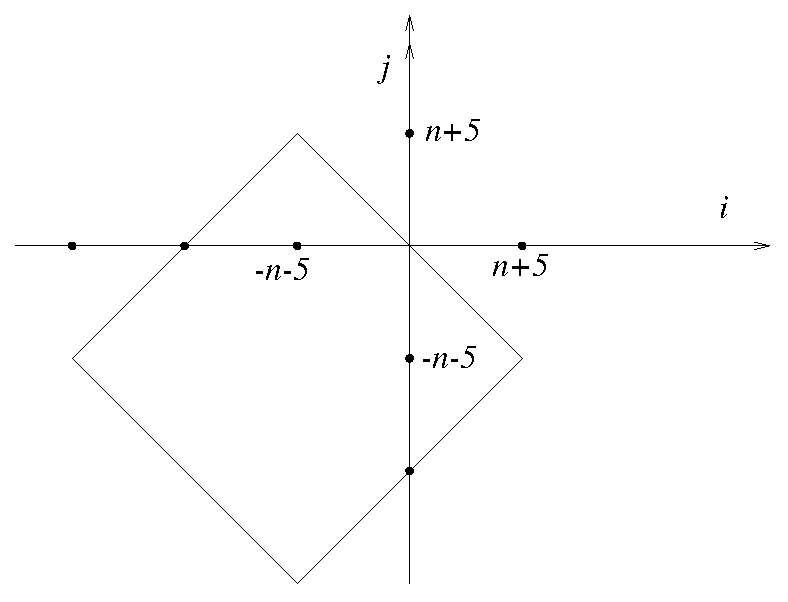
\includegraphics[height=6.5cm]{images/negatifs.eps}
\caption{\label{iter-domain} Problem domain}
\end{figure}
  
As above,
we introduce a new unknown $f$ and the inequality $f-i+2j \geq
0$. Since we want to optimize $f$, $f$ will appear
as the first unknown.

The trick for solving the problem in $Z$ is to introduce the following
parameters:
\begin{itemize}
\item $G \ge max(0, -i, -j, -f)$.
\item $P = max(0, -n)$.
\end{itemize}
This choice insure that the new variables and parameters:
\begin{eqnarray*}
f' &=& G + f \\
i' &=& G + i \\
j' &=& G + j \\
n' &=& P + n
\end{eqnarray*}
are all positive. This property stays true if $G$ grows. Hence, $G$
is again a big parameter. However, $P$ must be considered as an ordinary
parameter. After replacement of $i,j,n, f$ by the new variables
$i',j',n',f'$, we get a system which corresponds to the following input:

\begin{verbatim}
( 
 ( Solving MIN(i-2.j) under the following constraints:
   Unknowns may be negative.
   Order:
   f' i' j' constant G P n'
  )
 3 3 5 0 4 1
 ( 
  #[ 0 1 1 20 -2 -4 4 ]
  #[ 1 -1 2 0 -2 0 0 ]
  #[ 0 -1 -1 0 2 0 0 ]
  #[ 0 1 -1 10 0 -2 2 ]
  #[ 0 -1 1 10 0 -2 2 ]
   )
 ( ))
\end{verbatim}

The result is:
\begin{verbatim}
( 
 ( Solving MIN(i-2.j) under the following constraints:
   Unknowns may be negative.
   Order:
   f' i' j' constant G P n'
   -1 )(if #[ 0 -1 1 5]
(list #[ 1 3 -3 -15]
#[ 1 1 -1 -5]
#[ 1 -1 1 5]
)
()
)
)
\end{verbatim}
which should be read as:
\begin{eqnarray*}
 (f',i',j') & = & {\tt if}\;  -P+n'-5 \geq 0 \\
            &   & {\tt then} \; (G+3P-3n'-15, G+P-n'-5,G-P+n'+5) \\
            &   & {\tt else} \; \bot
\end{eqnarray*}
That is, in the original coordinate system:
\[ (f,i,j) = {\tt if}\;  n \geq 5 \; {\tt then} \; (-3n-15, -n-5, n+5)
 \; {\tt else} \; \bot \]
I.e., the minimum value for function $f$ is $-3n-15$, and this value
is reached at point $(-n-5, n+5)$. This minimum exists only if $n \ge 5$;
otherwise, the feasible set is empty.

\subsubsection{Mixed Programming}

A mixed program is a program in which some variables are constrained
to be integers while others may take rational values. Suppose for
instance that we have to solve:
\begin{eqnarray*}
S & = & \min a x + b y,\\
  &   & A x + B y + c \ge 0,
\end{eqnarray*}
where $y$ is the vector of the integer variables. First, solve

\begin{eqnarray*}
T & = & \min a x,\\
  &   & A x + B y + c \ge 0,
\end{eqnarray*}
in rational, with $y$ as parameters. The result is a quast.
To each leaf $i$ is associated a linear function $f_i(y)$
and a set of inequalities $C_i y + d_i \ge 0$. $T$ is equal to
$f_i$ when $y$ is such that the corresponding inequalities
are satisfied. For each $i$, solve the problem:
\begin{eqnarray*}
S_i & = & \min f_i(y) + b y,\\
  &   & C_i y + d_i \ge 0,
\end{eqnarray*}
in integers. The final result is the minimum of all $S_i$.
Obviously, the method can accomodate parameters in the
constraints. The $S_i$ will be functions of these
parameters, and the minimum must be computed symbolically.

%
% an example is needed here
%
\section{Using the PIP Library}
The PIP Library (PipLib for short) was implemented to allow the user to call PIP
directly from his programs, without file accesses or system calls. The
user only needs to link his programs with C libraries. The
PipLib mainly provides one function which takes as input the problem description
and some options, and returns a {\tt Quast} (see grammar \ref{GrammarOutputData}
in section \ref{OutputData}) corresponding to the solution. Some
other functions are provided for convenience reasons ; they
are described in section \ref{PipLibfunc}. Most of them require
some specific structures to represent the problem or
the solution ; these structures are described in section \ref{PipLibdata}.

\subsection{PipLib data structures description}\label{PipLibdata}
\subsubsection{PipMatrix structure}
\begin{verbatim}
struct pipmatrix
{ unsigned NbRows, NbColumns ;
  Entier ** p ;
  Entier * p_Init ;
  int p_Init_size ;
} ;
typedef struct pipmatrix PipMatrix ;
\end{verbatim}
The {\tt PipMatrix} structure is devoted to represent a constraints matrix in the
PolyLib shape \cite{Wild:93}. The whole matrix is arranged row after row at the
{\tt p\_Init} adress. {\tt p} is an array of pointers in which
{\tt p[i]} points to the beginning of the i$^{th}$ row.
{\tt NbRows} and {\tt NbColumns} are respectively the number of
rows and columns of the matrix. We use this structure to carry polyhedrons.
Each row corresponds to a constraint which the polyhedron must satisfy. The
constraint is an equality if the first element is $0$, an inequality 
$p(x) \geq 0$ if the first element is $1$. The next elements are
the unknown coefficients, followed by the parameter coefficients.
The last element is the constant factor.
For instance, in the problem of section \ref{exp2} the domain is defined by 3
constraints:
\begin{displaymath}
\left\{
\begin{array}{l}
-i + m \geq 0\\
-j + n \geq 0\\
j + i - k \geq 0
\end{array}
\right.
\end{displaymath}
the rows corresponding to these constraints would be:
\begin{verbatim}
# eq/in  i   j   k   m   n   cst
    1    0  -1   0   1   0    0 
    1   -1   0   0   0   1    0 
    1    1   1  -1   0   0    0 
\end{verbatim}
The context is defined by one constraint:
\begin{displaymath}
\left\{
\begin{array}{l}
-k + m + n \geq 0
\end{array}
\right.
\end{displaymath}
the row corresponding to this constraint would be:
\begin{verbatim}
# eq/in  k   m   n   cst
    1   -1   1   1    0 
\end{verbatim}
{\tt p\_Init\_size} is needed by the polylib to free the memory allocated by
mpz\_init in the multiple precision release.

\subsubsection{PipVector structure}
\begin{verbatim}
struct pipvector
{ int nb_elements ;
  Entier * the_vector ;
  Entier * the_deno ;
} ;
typedef struct pipvector PipVector ;
\end{verbatim}
The {\tt PipVector} structure represents a {\tt Vector}
as described in grammar \ref{GrammarOutputData} in section \ref{OutputData}.
{\tt nb\_elements} is the number of vector elements, {\tt the\_vector} is
an array which contains the numerators of these elements and {\tt the\_deno}
is an array which contains their denominators: the i$^{th}$ element is
{\tt the\_vector[i]/the\_deno[i]}.

\subsubsection{PipNewparm structure}
\begin{verbatim}
struct pipnewparm
{ int rank ;
  PipVector * vector ;
  Entier deno ;
  struct pipnewparm * next ;
} ;
typedef struct pipnewparm PipNewparm ;
\end{verbatim}
The {\tt PipNewparm} structure represents a {\tt NULL} terminated linked list of
{\tt Newparm} as described in grammar \ref{GrammarOutputData}
in section \ref{OutputData}. For each {\tt Newparm}, the rank is {\tt rank},
the vector of coefficients is pointed by {\tt vector}, and the denominator
is {\tt deno}. {\tt next} is a pointer to the next {\tt PipNewparm} structure.

\subsubsection{PipList structure}
\begin{verbatim}
struct piplist
{ PipVector * vector ;
  struct piplist * next ;
} ;
typedef struct piplist PipList ;
\end{verbatim}
The {\tt PipList} structure represents a {\tt NULL} terminated linked list of
{\tt Vector} as described in grammar \ref{GrammarOutputData} in section
\ref{OutputData}. {\tt vector} is a pointer to the vector of the current node and
{\tt next} is a pointer to the next {\tt PipList} structure.

\subsubsection{PipQuast structure}
\begin{verbatim}
struct pipquast
{ PipNewparm * newparm ;
  PipList * list ;
  PipVector * condition ;
  struct pipquast * next_then ;
  struct pipquast * next_else ;
  struct pipquast * father ;
} ;      
typedef struct pipquast PipQuast ;
\end{verbatim}
The {\tt PipQuast} represents a {\tt Quast} as described in
grammar \ref{GrammarOutputData} in section \ref{OutputData}. Each {\tt Quast}
has a tree structure and begins with a list of {\tt Newparm}
(field {\tt newparm}). If the pointer {\tt condition} is not {\tt NULL}, the
list of {\tt Newparm} is followed by a conditional structure : if the condition
pointed by {\tt condition} is true, then the solution continues in the
{\tt Quast} pointed by {\tt next\_then}, in the {\tt Quast} pointed by
{\tt next\_else} otherwise. If the pointer {\tt condition} is {\tt NULL}, the
list of {\tt Newparm} is followed by a list of vectors (field {\tt list}).
For {\tt Quast} manipulation convenience, a pointer to the father in the tree
is provided (field {\tt father}), obviously the father of the root is {\tt NULL}. 


\subsubsection{PipOptions structure}
\begin{verbatim}
struct pipoptions
{ int Nq ;
  int Verbose ;
  int Simplify ;
  int Deepest_cut ;
  int Maximize;
  int Urs_unknowns;
} ;      
typedef struct pipoptions PipOptions ;
\end{verbatim}
The {\tt PipOptions} structure contains all the possible options ruling
the PIP behaviour and having to be set by the user: 
\begin{enumerate}
\item {\tt Nq}: a boolean set to 1 if an integer solution is needed, 0
      otherwise,
\item {\tt Verbose}: a graduate value for debug informations:
      \begin{itemize}
      \item -1: absolute silence,
      \item 0: relative silence,
      \item 1: information on cuts when an integer solution is required,
      \item 2: information on pivots and determinants,
      \item 3: information on arrays.
      \end{itemize}
      Each option include the preceding one.
      If {\tt Verbose} is not $-1$, most of the processing will be printed in
      a file. The file name is generated at random (by \textit{mkstemp}) or
      set with environment variable DEBUG.
\item {\tt Simplify}: a boolean set to 1 if some trivial quast simplifications
      are needed (recursive elimination of degenerated patterns like
      {\tt if \#[...] () ()}), 0 otherwise,
\item {\tt Deepest\_cut}: a boolean set to 1 if PIP has to use the deepest cut
      algorithm, 0 otherwise,
\item {\tt Maximize}: a boolean set to 0 if the lexicographic
      minimum is requested, or to 1 for the lexicographic maximum. When trying to
      find the lexicographic maximum, the method used is the one
      presented in Section~\ref{maximum}: if no bigparm was set, a new (big)
      parameter is automatically created by adding a new ending column to the
      constraint system.  This optional extra parameter is removed again from the
      output.  Unbounded solutions have their \verb+the_deno+ set to zero.
      Note that setting this option allows for negative solutions.
      This may change in a future release.
\item \verb+Urs_unknowns+: controls signs of unknowns:
	\begin{itemize}
	\item -1: all unknowns have unrestricted sign,
	\item 0: all unknowns are non-negative.
        \end{itemize}
\end{enumerate}
Every {\tt PipOptions} structure should be created and filled with the default
values by the {\tt pip\_options\_init} function (see section \ref{optinit}).

\subsection{PipLib functions description}\label{PipLibfunc}
\subsubsection{pip\_solve function}
\begin{verbatim}
PipQuast * pip_solve
( PipMatrix * domain,
  PipMatrix * context,
  int Bg,
  PipOptions * options
) ;
\end{verbatim}
The {\tt pip\_solve} function solves a linear problem provided as input. The
first three parameters describe the problem that the user wants to solve.
The last parameter describe the options that the user has to set.
These parameters are:
\begin{enumerate}
\item {\tt domain}: a pointer to the equations and inequations system which
      describes the unknown domain in the PolyLib constraints matrix shape,
\item {\tt context}: a pointer to the equations and inequations system satisfied
      by the parameters context in the PolyLib constraints matrix shape
      (it can be NULL if there is no context),
\item {\tt Bg}: the column rank of the bignum (first column rank is 0), or a
      negative value if there is no big parameter in the problem to be solved, 
\item {\tt options}: a pointer to a data structure containing the options
      ruling the behaviour of PIP.
\end{enumerate}
This function returns a pointer to a {\tt PipQuast} structure containing the
solution, it will be {\tt NULL} if the context is {\tt void}.

\subsubsection{pip\_options\_init function}\label{optinit}
\begin{verbatim}
PipOptions * pip_options_init(void) ;
\end{verbatim}
The {\tt pip\_options\_init} function allocates the memory space for a
{\tt PipOptions} structure and fills it with the default values:
\begin{itemize}
\item {\tt Nq} $= 1$: an integer value is required,
\item {\tt Verbose} $= 0$: no debug informations,
\item {\tt Simplify} $= 0$: do not try to simplify solutions,
\item {\tt Deepest\_cut} $= 0$: do not use deepest cut algorithm,
\item {\tt Maximize} $= 0$: compute the lexicographic minimum,
\item \verb+Urs_unknowns+ $= 0$: all unknowns are non-negative.
\end{itemize}
We strongly recommand to use this function to create and initialize any
{\tt PipOptions} structure. In this way, if some new options appear in
the future, there will be no compatibility problems.

\subsubsection{pip\_close function}
\begin{verbatim}
void pip_close(void) ;
\end{verbatim}
The {\tt pip\_close} frees the memory space that have been allocated for
few global variables PipLib needs. This function has to be called when
PipLib is no more useful in order to prevent slight memory leaks.

\subsubsection{pip\_matrix\_alloc function}
\begin{verbatim}
PipMatrix * pip_matrix_alloc
( unsigned nb_rows,
  unsigned nb_columns
) ;
\end{verbatim}
The {\tt pip\_matrix\_alloc} function allocates the memory space
for a {\tt PipMatrix} structure with {\tt nb\_rows} rows and {\tt nb\_columns}
columns. It fills the {\tt Nb\_Rows}, {\tt Nb\_Columns} and {\tt p} fields
and initializes the matrix entries to 0, then it returns a pointer to this
structure.

\subsubsection{pip\_matrix\_read function}
\begin{verbatim}
PipMatrix * pip_matrix_read(FILE *) ;
\end{verbatim}
The {\tt pip\_matrix\_read} function read a matrix from a file. It takes
as input a pointer to the file it has to read (possibly {\tt stdin}), and
returns a pointer to a {\tt PipMatrix} structure. The input has the following syntax:
\begin{itemize}
\item some optional comment lines which begin with {\tt \#},
\item the row numbers and column numbers, possibly followed by comments,
      on a single line,
\item the matrix rows, each row must be on a single line and is possibly
      followed by comments.
\end{itemize}
For instance, in the problem of section \ref{exp2} the domain is defined as follows
\begin{verbatim}
# This is the domain
3 7                 # 3 lines and 7 columns
1  0 -1  0  1  0  0 # -i + m >= 0
1 -1  0  0  0  1  0 # -j + n >= 0
1  1  1 -1  0  0  0 # j + i - k >= 0
\end{verbatim}

\subsubsection{Printing Functions}
\begin{verbatim}
void pip_matrix_print(FILE *, PipMatrix *) ;
void pip_vector_print(FILE *, PipVector *) ;
void pip_newparm_print(FILE *, PipNewparm *, int indent) ;
void pip_list_print(FILE *, PipList *, int indent) ;
void pip_quast_print(FILE *, PipQuast *, int indent) ;
void pip_options_print(FILE *, PipOptions *) ;
\end{verbatim}
There is a printing function for each structure of the PipLib. They all take as input
a pointer to a file (possibly {\tt stdout}) and a pointer to a structure.
Some of them takes as input an
indent step. They print the structure contents to the file without indent if
{\tt indent} $< 0$, with an indentation step of {\tt indent} otherwise.

\subsubsection{Memory Deallocation Functions}
\begin{verbatim}
void pip_matrix_free(PipMatrix *) ;
void pip_vector_free(PipVector *) ;
void pip_newparm_free(PipNewparm *) ;
void pip_list_free(PipList *) ;
void pip_quast_free(PipQuast *) ;
void pip_options_free(PipOptions *) ;
\end{verbatim}
There is a memory deallocation function for each structure of the PipLib.
They free the allocated memory for the structure.

\subsection{Example}
Here is a simple example showing how one can use the PipLib, assuming that
a basic installation was done. The following C program reads a domain and its
context on the standard input then prints the solution on the standard output.
Options are preselected : there is no bignum, we are looking for an integral
solution without simplification and we don't want debug informations.
\begin{verbatim}
/* example.c */
# include <stdio.h>
# include <piplib/piplib64.h>

int main()
{ PipMatrix * domain, * context  ;
  PipQuast * solution ;
  PipOptions * options ;
 
  domain = pip_matrix_read(stdin) ;
  context = pip_matrix_read(stdin) ;
  options = pip_options_init() ;

  solution = pip_solve(domain,context,-1,options) ;

  pip_options_free(options) ;
  pip_matrix_free(domain) ;
  pip_matrix_free(context) ;

  pip_quast_print(stdout,solution,0) ;
  pip_close() ;
}
\end{verbatim}
The compilation command could be :
\begin{verbatim}
gcc example.c -lpiplib64 -o example
\end{verbatim}
Supposing that the user wants to solve the problem of section \ref{exp2}, he
will type:
\begin{verbatim}
3 7
1  0 -1  0  1  0  0 
1 -1  0  0  0  1  0 
1  1  1 -1  0  0  0 
1 5
1 -1  1  1  0 
\end{verbatim}
And the program will print :
\begin{verbatim}
(if #[ -1 1 0 0]
 (list
  #[ 0 0 0 0]
  #[ 1 0 0 0]
 )
 (list
  #[ 1 -1 0 0]
  #[ 0 1 0 0]
 )
)
\end{verbatim}

\section{Installing PIP}

\subsection{Implementation Notes}

The main problem with any integer programming software is that, since one
must distinguish between integer and rationals, all computations are
to be done exactly. Rationals must be represented as quotients with
an integer numerator and an integer denominator. In the preceding version,
there was only one denominator for the whole tableau. The consequence
was that simplifications where most unlikely, and that the integers
in the tableau were growing until overflows occured.

In the present version, there is one denominator per row of the tableau.
Reduction to lower terms occurs frequently, and the growth of numbers in the
problem tableau is limited. As a consequence, much larger problems can be
solved. This has had the unfortunate consequence that several bugs, which
were beyond the domain of the old version, have now surfaced. These bugs
have been corrected. As far as the author
 can tell, these bugs mainly gave correct
results which were not in simplest form: the quast had extraneous leaves.
In some cases, the result was wrong but the error was self evident: for 
instance, there were denominators in integer results.

\subsection{License}
This program is free software; you can redistribute it and/or
modify it under the terms of the GNU General Public License version 2
as published by the Free Software Foundation.

This program is distributed in the hope that it will be useful,
but WITHOUT ANY WARRANTY; without even the implied warranty of
MERCHANTABILITY or FITNESS FOR A PARTICULAR PURPOSE.  See the
GNU General Public License for more details.
{\tt http://www.gnu.org/copyleft/gpl.html}

\subsection{Adjusting the Precision}
Pip is an all integer  version of the dual simplex algorithm. As such,
it has to handle integers whose size may grow exponentially as the
computation proceeds. Integer overflow may occur and have to be checked.
Since the hardware integer overflow exception is usually masked by
the operating system or the compiler, overflow is detected by checking
that a division somewhere in the algorithm, which can be proved to be
exact by mathematical arguments, is indeed exact. If not, an error is
reported and the computation stops.

The size of the numbers to be handled depends strongly on the size of the
constraint matrix and on the size of its coefficients.

\subsubsection{Bounded Pip}
The precision of the integer representation in the Pip code can be
adjusted at compile time by giving options to the {\tt configure}
shell script.
By giving {\tt configure} the option {\tt --enable-llint} you ask
for long long int version only (64 bits). It results in a 64 bits Pip
called {\tt pip64}.
By giving {\tt configure} the option {\tt --enable-int} you
ask for int version only. It results in a 32 bits called
{\tt pip32} and a faster running time.

\subsubsection{Multiple Precision Pip}
Multiple Precision Pip is built on top of the GMP library
(this library is freely available at {\tt http://www.swox.com/gmp}). 
Each integer in the program is represented as a list of 32 bits numbers.
All computations are done exactly, and the size of the numbers increases
as needed to preserve exactness. It follows that no overflow is possible.
However, when the size of numbers increases, computations get slower and
slower, and memory overflow may occur in extreme cases. In well behaved
problems, 32 bits are enough for the initial data, the size of intermediate
results first increases up to a maximum, then decreses, and 32 bits
are again enough for the results. Hence, it has been possible to keep
the input format and output format of Multiple Precision Pip completely
compatible with the formats of the bounded precision versions.

To install Multiple Precision Pip, first install Gmp according to the
directions found at the above URL. Usually, the library is installed
in {\tt /usr/local/lib}, and the header files are in {\tt /usr/local/include}.
If this is not the case, you must adjust the Pip makefile by giving
to the {\tt configure} shell script the option {\tt --with-gmp=PATH}, where
{\tt PATH} is the GMP library installation path.

By giving {\tt configure} the option {\tt --enable-gmp} you ask
for a GMP version only. It results in a multiple precision Pip
called {\tt pipMP}.


\subsection{Building the Executable and the Library}

To build PIP, first copy the above tarfile to any convenient directory.
Expand the tarfile using:
\begin{verbatim}
zcat pip.tar.Z | tar xvf -
\end{verbatim}
You should obtain the following files:
\begin{itemize}
\item header files in the {\tt include} directory,
\item C code files in the {\tt source} directory,
\item a lot of data files {\tt *.dat} and of result files {\tt *.ll}
      in the {\tt test} directory (you should then run at least some of
      the {\tt *.dat} files and compare the results to the corresponding
      {\tt *.ll} file),
\item a simple example showing how to use the PipLib in the {\tt example} directory,
\item a postscript version of the present document, {\tt pip.ps} in the
      {\tt doc} directory,
\item files needed for compilation and installation in the PIP
      root directory.
\end{itemize}


\subsubsection{basic installation}

The {\tt configure} shell script attempts to guess correct values for
various system-dependent variables used during compilation.  It uses
those values to create a {\tt Makefile}.
The file {\tt configure.in} is used to create {\tt configure} by a program
called {\tt autoconf}.  You only need {\tt configure.in} if you want to change
it or regenerate {\tt configure} using a newer version of {\tt autoconf}.

The simplest way to compile this package is:
\begin{itemize}
\item {\tt cd} to the directory containing the package's source code and type \linebreak
      {\tt ./configure} to configure the package for your system
      (while running, {\tt configure} prints some
      messages telling which features it is checking for),

\item type {\tt make} to compile the package and install the program and the
      library,

\item you can remove the program binaries and object files from the
      source code directory by typing {\tt make clean}. To also remove the
      files that {\tt configure} created (so you can compile the package for
      a different kind of computer) type {\tt make distclean}.
\end{itemize}

PIP and the PipLib have been successfully compiled on the following systems:
\begin{itemize}
\item PC's under Linux, with the {\tt gcc} compiler,
\item PC's under Windows (Cygwin), with the {\tt gcc} compiler (but because
of some Cygwin limitations, only 32 bits version will work and user may
experience some problems when linking with PipLib),
\item SparcStations, with the {\tt gcc} compiler.
\end{itemize}

\subsubsection{optionnal features}   

\begin{itemize}
\item By default, {\tt make} will install the package's files in
{\tt /usr/local/bin}, \linebreak {\tt /usr/local/lib}, etc. You can specify an
installation prefix other than {\tt /usr/local} by giving {\tt configure} the
option {\tt --prefix=PATH}.

\item By default, both PIP and the PipLib are compiled and installed. By giving
{\tt configure} the option {\tt --without-pip} you disable the compilation and
installation of PIP. By giving {\tt configure} the option {\tt --without-lib}
you disable the compilation and installation of the PipLib.

\item By default, both int (32 bits) and long long int (64 bits) versions are
built. Multiple precision is built too if the GMP library is found.
By giving {\tt configure} the option {\tt --enable-int} you ask for int
version only. By giving {\tt configure} the option {\tt --enable-llint} you
ask for long long int version only. By giving {\tt configure} the
option {\tt --enable-gmp} you ask for GMP version only.

\item By default, PIP looks for the GMP library in the standard path
({\tt /usr/} or {\tt /usr/local/}). If the multiple precision Pip construction
is needed and if the GMP library was installed elsewhere, you must must give
to the {\tt configure} shell script the option {\tt --with-gmp=PATH}, where
{\tt PATH} is the GMP library installation path. Another possibility is to
give the GMP include and/or library path separately by using 
{\tt --with-gmp-include=PATH} and {\tt --with-gmp-library=PATH}.
\end{itemize}

\subsubsection{uninstallation}
You can easily remove PIP and the PipLib from your system by typing
{\tt make uninstall}.

\vspace{0.5cm}
Report all bugs, problems, inaccuracies in the documentation to:

{\tt Paul.Feautrier@ens-lyon.fr}

{\tt Cedric.Bastoul@prism.uvsq.fr}

Praise is also appreciated.

Let the power of parametric integer programming be with you.

\bibliography{%
/users/prism/pf/local/biblio/totale%
,/users/prism/pf/local/biblio/second%
,/users/prism/pf/local/biblio/quater%
}

\end{document}
